\documentclass{article}\usepackage[]{graphicx}\usepackage[]{color}
%% maxwidth is the original width if it is less than linewidth
%% otherwise use linewidth (to make sure the graphics do not exceed the margin)
\makeatletter
\def\maxwidth{ %
  \ifdim\Gin@nat@width>\linewidth
    \linewidth
  \else
    \Gin@nat@width
  \fi
}
\makeatother

\definecolor{fgcolor}{rgb}{0.345, 0.345, 0.345}
\newcommand{\hlnum}[1]{\textcolor[rgb]{0.686,0.059,0.569}{#1}}%
\newcommand{\hlstr}[1]{\textcolor[rgb]{0.192,0.494,0.8}{#1}}%
\newcommand{\hlcom}[1]{\textcolor[rgb]{0.678,0.584,0.686}{\textit{#1}}}%
\newcommand{\hlopt}[1]{\textcolor[rgb]{0,0,0}{#1}}%
\newcommand{\hlstd}[1]{\textcolor[rgb]{0.345,0.345,0.345}{#1}}%
\newcommand{\hlkwa}[1]{\textcolor[rgb]{0.161,0.373,0.58}{\textbf{#1}}}%
\newcommand{\hlkwb}[1]{\textcolor[rgb]{0.69,0.353,0.396}{#1}}%
\newcommand{\hlkwc}[1]{\textcolor[rgb]{0.333,0.667,0.333}{#1}}%
\newcommand{\hlkwd}[1]{\textcolor[rgb]{0.737,0.353,0.396}{\textbf{#1}}}%

\usepackage{framed}
\makeatletter
\newenvironment{kframe}{%
 \def\at@end@of@kframe{}%
 \ifinner\ifhmode%
  \def\at@end@of@kframe{\end{minipage}}%
  \begin{minipage}{\columnwidth}%
 \fi\fi%
 \def\FrameCommand##1{\hskip\@totalleftmargin \hskip-\fboxsep
 \colorbox{shadecolor}{##1}\hskip-\fboxsep
     % There is no \\@totalrightmargin, so:
     \hskip-\linewidth \hskip-\@totalleftmargin \hskip\columnwidth}%
 \MakeFramed {\advance\hsize-\width
   \@totalleftmargin\z@ \linewidth\hsize
   \@setminipage}}%
 {\par\unskip\endMakeFramed%
 \at@end@of@kframe}
\makeatother

\definecolor{shadecolor}{rgb}{.97, .97, .97}
\definecolor{messagecolor}{rgb}{0, 0, 0}
\definecolor{warningcolor}{rgb}{1, 0, 1}
\definecolor{errorcolor}{rgb}{1, 0, 0}
\newenvironment{knitrout}{}{} % an empty environment to be redefined in TeX

\usepackage{alltt}
%this is a comment

\usepackage{graphicx}
%\DeclareGraphicsExtensions{.png,.jpg}

\newcommand{\dataframe}{\texttt{data.frame}}

\author{Z. Berkay Celik}
\title{ Introduction to Latex using RStudio and Knitr}
\date{July 4th 2014}
\IfFileExists{upquote.sty}{\usepackage{upquote}}{}
\begin{document}
\maketitle
\tableofcontents

\section{Section 1}
\label{sec:section1}
This is the first section for introduction, we talk about \dataframe{}s.

This tutorial is a first step for \textit{R}.

\section{Section 2}
\label{section2}
In Section~\ref{sec:section1} we have covered some basics, now key point is how to include r codes as well as graphics.

\subsection{R codes}
In this subsection, we will look Diamonds data.All R code goes in between.
\begin{knitrout}
\definecolor{shadecolor}{rgb}{0.969, 0.969, 0.969}\color{fgcolor}\begin{kframe}
\begin{alltt}
\hlcom{#Now, we can write our R code.}
\hlkwd{require} \hlstd{(ggplot2)}
\end{alltt}


{\ttfamily\noindent\itshape\color{messagecolor}{\#\# Loading required package: ggplot2}}

{\ttfamily\noindent\color{warningcolor}{\#\# Warning: package 'ggplot2' was built under R version 3.0.3}}\begin{alltt}
\hlkwd{data}\hlstd{(diamonds)}
\hlkwd{head}\hlstd{(diamonds)}
\end{alltt}
\begin{verbatim}
##   carat       cut color clarity depth table price    x    y    z
## 1  0.23     Ideal     E     SI2  61.5    55   326 3.95 3.98 2.43
## 2  0.21   Premium     E     SI1  59.8    61   326 3.89 3.84 2.31
## 3  0.23      Good     E     VS1  56.9    65   327 4.05 4.07 2.31
## 4  0.29   Premium     I     VS2  62.4    58   334 4.20 4.23 2.63
## 5  0.31      Good     J     SI2  63.3    58   335 4.34 4.35 2.75
## 6  0.24 Very Good     J    VVS2  62.8    57   336 3.94 3.96 2.48
\end{verbatim}
\begin{alltt}
\hlstd{mod1} \hlkwb{<-} \hlkwd{lm}\hlstd{(price} \hlopt{~} \hlstd{carat,} \hlkwc{data} \hlstd{= diamonds)}
\hlkwd{summary}\hlstd{(mod1)}
\end{alltt}
\begin{verbatim}
## 
## Call:
## lm(formula = price ~ carat, data = diamonds)
## 
## Residuals:
##    Min     1Q Median     3Q    Max 
## -18585   -805    -19    537  12732 
## 
## Coefficients:
##             Estimate Std. Error t value Pr(>|t|)    
## (Intercept)  -2256.4       13.1    -173   <2e-16 ***
## carat         7756.4       14.1     551   <2e-16 ***
## ---
## Signif. codes:  0 '***' 0.001 '**' 0.01 '*' 0.05 '.' 0.1 ' ' 1
## 
## Residual standard error: 1550 on 53938 degrees of freedom
## Multiple R-squared:  0.849,	Adjusted R-squared:  0.849 
## F-statistic: 3.04e+05 on 1 and 53938 DF,  p-value: <2e-16
\end{verbatim}
\end{kframe}
\end{knitrout}
Scatter plot of carat vs.price is plotted in Figure \ref{fig:diamonds-plot} by using geomsmooth
\begin{knitrout}
\definecolor{shadecolor}{rgb}{0.969, 0.969, 0.969}\color{fgcolor}\begin{kframe}
\begin{alltt}
\hlkwd{ggplot}\hlstd{(}\hlkwc{data}\hlstd{=diamonds,} \hlkwd{aes}\hlstd{(}\hlkwc{x}\hlstd{=carat,} \hlkwc{y}\hlstd{=price,} \hlkwc{color}\hlstd{=color))}\hlopt{+} \hlkwd{geom_point}\hlstd{()} \hlopt{+} \hlkwd{geom_smooth}\hlstd{(}\hlkwc{method}\hlstd{=}\hlstr{"lm"}\hlstd{)}
\end{alltt}
\end{kframe}\begin{figure}[]

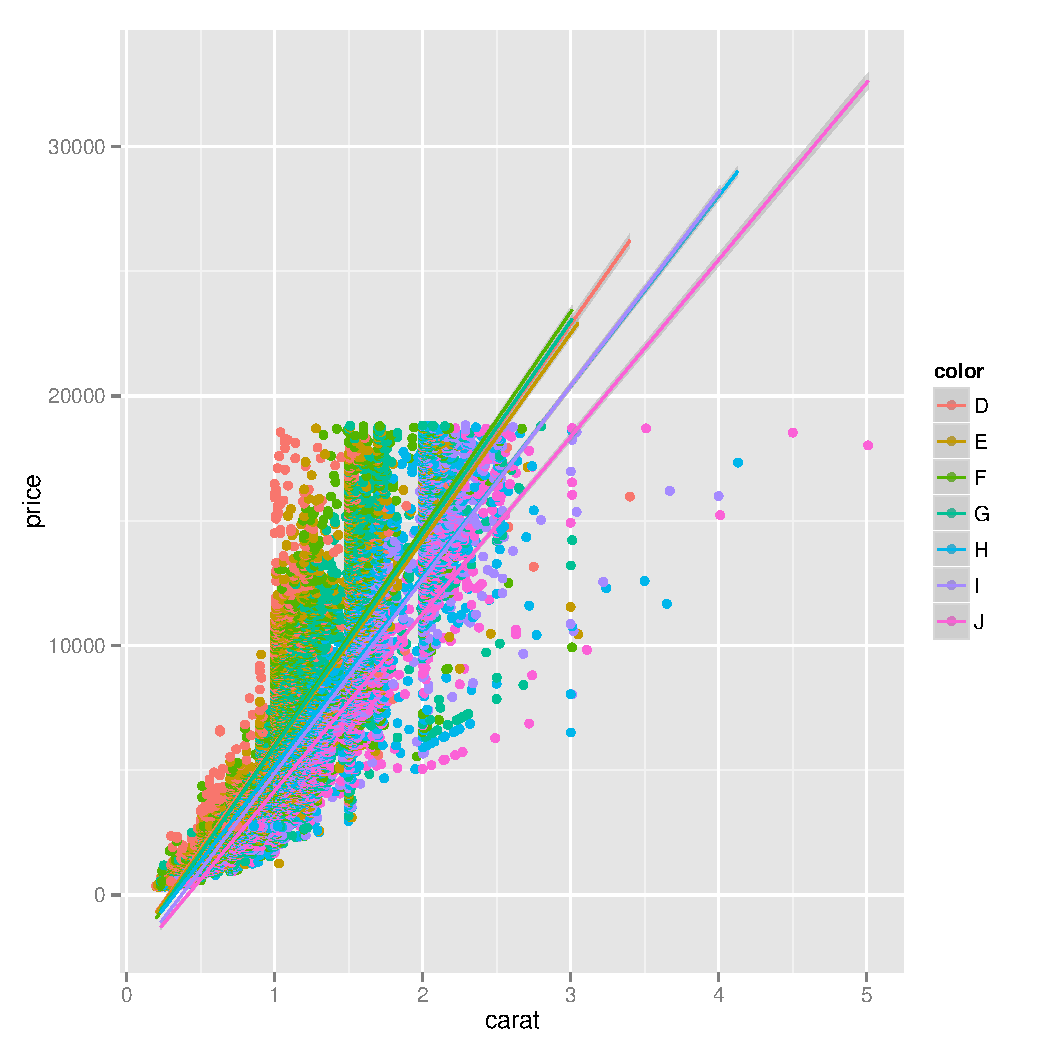
\includegraphics[width=.95\linewidth]{figure/diamonds-plot} \caption[Scatterplot of carat vs]{Scatterplot of carat vs. price\label{fig:diamonds-plot}}
\end{figure}


\end{knitrout}


\begin{knitrout}
\definecolor{shadecolor}{rgb}{0.969, 0.969, 0.969}\color{fgcolor}\begin{kframe}
\begin{alltt}
\hlkwd{ggplot}\hlstd{(}\hlkwc{data}\hlstd{=diamonds,} \hlkwd{aes}\hlstd{(}\hlkwc{x}\hlstd{=carat,}\hlkwc{y}\hlstd{=price,} \hlkwc{color}\hlstd{=color))} \hlopt{+} \hlkwd{geom_point}\hlstd{()} \hlopt{+} \hlkwd{xlab}\hlstd{(}\hlstr{"carats"}\hlstd{)}
\end{alltt}
\end{kframe}\begin{figure}[]

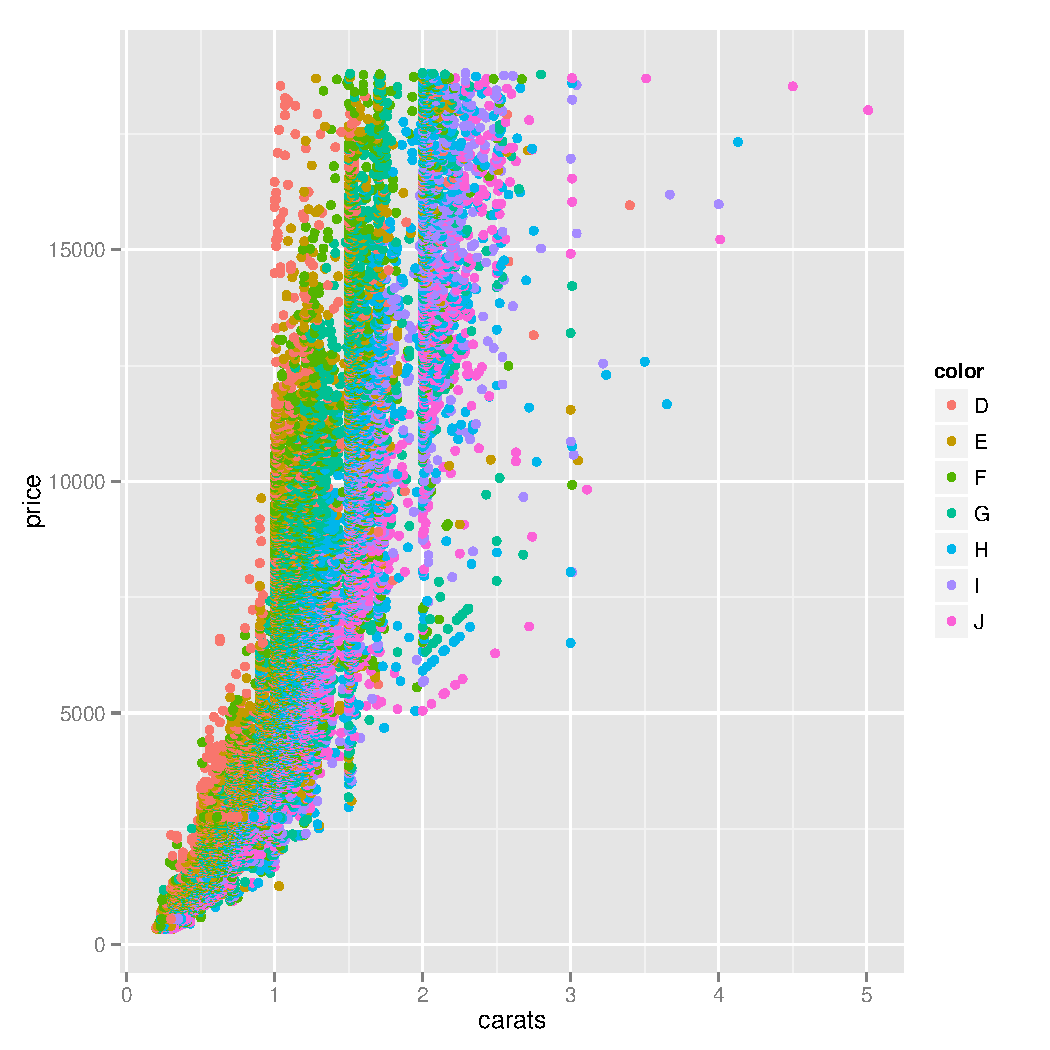
\includegraphics[width=.95\linewidth]{figure/diamonds-plot2} \caption[Scatterplot of diamonds]{Scatterplot of diamonds\label{fig:diamonds-plot2}}
\end{figure}


\end{knitrout}

\end{document}
